\section{Descripci�n del modelo IEC 61850 orientado a objetos mediante SCL}
El \gls{SCL}, como se ha mencionado 
en los cap�tulos introductorios,
define b�sicamente 5 grandes partes:
\begin{enumerate}
  \item Header
  \item Substation
  \item Communication
  \item IED
  \item DataTypeTemplates 
\end{enumerate}  
La representaci�n en \gls{UML-es} de estas 5
partes mencionadas es presentada en la 
figura \ref{fig:SCL-main-parts}.
 
\begin{figure}
\begin{center}
  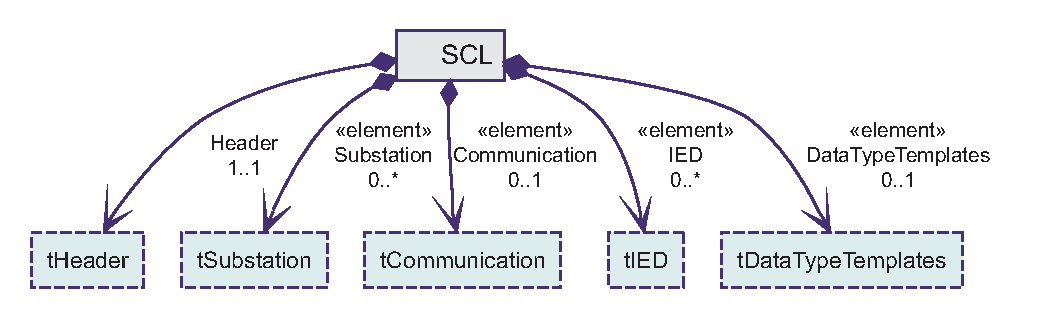
\includegraphics[width=1.0\textwidth]{chapters/enfoque/figures/scl-depth2-heredado.eps}
  \caption{Partes principales del SCL}
  \label{fig:SCL-main-parts}
\end{center}
\end{figure}

Antes de explicar estas partes 
con la profundidad adecuada, 
es necesario 
formular una definici�n precisa 
del paradigma \gls{O-O-es}. Muchos 
autores ya han formulado definiciones 
precisas  
\cite{Rentsch:1982} 
\cite{Pascoe:1986}
\cite{Nygaard:1986}
\cite{Madsen:1988}, 
y la definici�n de Lastly, Wegner
\cite{Wegner:1987} ha sido 
la m�s aceptada \cite{Capretz:2003}.
Wegner define el paradigma \gls{O-O-es} 
en t�rminos de objetos, clases y herencia.

\emph{
	`` Los objetos son entidades aut�nomas
	que responden a mensajes u operaciones y
	comparten un estado. Las clases clasifican
	objetos por sus operaciones comunes.
	La herencia sirve para clasificar clases 
	con respecto a su comportamiento com�n. La 
	abstracci�n de datos esconde (simplifica) la 
	representaci�n de datos y su implementaci�n 
	de operaciones '' 
}\cite{Wegner:1987}. Esto es: 

\begin{center}
	orientado a objetos = objetos + clases + herencia
\end{center}

%Estos conceptos En las siguientes secciones

La metodolog�a que utiliz� la norma IEC 61850 
para la creaci�n del \gls{SCL} y los modelos de 
informaci�n definidos formalmente en IEC 61850--7--x 
\cite{IEC61850-7-1:2003}
\cite{IEC61850-7-2:2003}
\cite{IEC61850-7-3:2003}
\cite{IEC61850-7-4:2003}
\cite{IEC61850-7-410:2007} 
enfoca la organizaci�n del modelo
a trav�s de la creaci�n de objetos de la siguiente forma:
Los objetos guardan el dato y tienen un 
comportamiento propio con una forma particular 
para agrupar la informaci�n por funcionalidades comunes 
y estructuras comunes de la informaci�n. 
Este enfoque permite 
empaquetar un conjunto de acciones comunes,
manejar una peque�a cantidad de variables 
en lugar de m�ltiples variables, 
organizar comportamientos comunes agrup�ndolos 
y estructurando los 
sistemas l�gicos de forma a que 
representen al mundo real.



%\subsubsection{Clases}
%\subsubsection{Objetos}




